% =============================================================================
%  Cifra — Informe final de Matemáticas Discretas
%  Compilar:  pdflatex informe.tex   (dos veces, para el índice)
%  Necesita la carpeta figuras/ al lado de este archivo.
% =============================================================================
\documentclass[12pt,letterpaper]{article}

\usepackage[T1]{fontenc}
\usepackage[utf8]{inputenc}
% En una instalación normal de LaTeX (Overleaf, TeX Live, MiKTeX) se usa babel en
% español, que trae la partición de palabras correcta. Si el paquete del idioma no
% está instalado, el documento sigue compilando con los rótulos puestos a mano.
\IfFileExists{spanish.ldf}{%
  \usepackage[spanish,es-tabla,es-noquoting]{babel}%
}{%
  \renewcommand{\contentsname}{Índice}%
  \renewcommand{\figurename}{Figura}%
  \renewcommand{\tablename}{Tabla}%
  \renewcommand{\appendixname}{Anexo}%
  \renewcommand{\refname}{Referencias}%
}
\usepackage{lmodern}
\usepackage[margin=2.7cm]{geometry}
\usepackage{amsmath,amssymb}
\usepackage{graphicx}
\usepackage{booktabs}
\usepackage[font=small,labelfont=it,labelsep=period]{caption}
\usepackage{subcaption}
\usepackage{enumitem}
\usepackage{float}
\usepackage{microtype}
\usepackage[hidelinks]{hyperref}
\usepackage{url}
\urlstyle{tt}
\Urlmuskip=0mu plus 1mu              % deja que las direcciones largas se partan

\setlist[itemize]{itemsep=2pt,topsep=4pt,parsep=0pt}
\setlist[enumerate]{itemsep=2pt,topsep=4pt,parsep=0pt}
\renewcommand{\arraystretch}{1.15}

% Las figuras son anchas y van ancladas a su apartado: se le da a LaTeX mucho
% margen para colocarlas donde toca y poco para mandarlas al final.
\renewcommand{\topfraction}{0.92}
\renewcommand{\bottomfraction}{0.75}
\renewcommand{\textfraction}{0.08}
\renewcommand{\floatpagefraction}{0.75}

\newcommand{\pc}{\,\%}

\title{Cifra}
\author{}
\date{}

\begin{document}

% ------------------------------------------------------------------ portada --
\begin{titlepage}
\centering
\vspace*{3.2cm}

{\Huge\bfseries Cifra\par}
\vspace{0.9cm}
{\Large Reconocimiento de dígitos manuscritos con una red neuronal,\\[2pt]
desde la matemática discreta\par}

\vspace{2.6cm}
{\large Santiago Zelaya \quad Santiago Rincón \quad Isabella Rodríguez \quad José Daza\par}

\vspace{2.2cm}
{\large Matemáticas Discretas (MAT 4021)\par}
\vspace{0.3cm}
{\large Docente: MSc. Iván Gómez\par}

\vspace{1.4cm}
{\large Universidad del Norte\par}
{\large Barranquilla, Colombia\par}

\vfill
{\large 16 de noviembre de 2026\par}
\end{titlepage}

\pagenumbering{roman}
\tableofcontents
\newpage
\pagenumbering{arabic}

% ------------------------------------------------------------------ resumen --
\section{Resumen}

Este proyecto construye \textbf{Cifra}, una aplicación web en la que una persona
escribe un número a mano, con el dedo o con un lápiz digital, y una red neuronal
lo lee en el mismo dispositivo, sin enviar nada a ningún servidor. La aplicación
tiene dos usos: practicar la escritura de números y sumar una cuenta escrita a
mano, como la caja de una tienda de barrio.

El interés para la asignatura no está solo en que la red funcione, sino en que el
problema se deja describir por completo con herramientas de matemática discreta.
Un dibujo de $28\times28$ píxeles es una matriz binaria; la diferencia entre dos
dibujos es la distancia de Hamming, que coincide con la cantidad de unos de su
disyunción exclusiva; el conjunto de todos los dibujos posibles tiene cardinalidad
$2^{784}$; la relación «representar el mismo dígito» es de equivalencia y parte
ese conjunto en diez clases; y la razón por la que la red necesita capas ocultas
es la misma por la que un perceptrón de umbral no resuelve la función XOR.

La red final, de 784 entradas, dos capas ocultas de 128 y 48 neuronas y 10
salidas, alcanza una exactitud de $96.65\pc$ sobre un conjunto de prueba de 2000
imágenes que nunca vio. Como contraste, un clasificador puramente discreto que
solo compara píxel a píxel con la distancia de Hamming llega a $86.80\pc$, y una
regresión logística sin capas ocultas a $90.45\pc$. La aplicación incluye un panel
que muestra las activaciones de cada neurona, el cálculo con los números del
dibujo actual y la parte discreta, lo que permite sustentar el funcionamiento
interno y no solo el resultado.

% ------------------------------------------------------------- introducción --
\section{Introducción}

\subsection{El problema}

Escribir números a mano es más rápido y más natural que teclearlos, sobre todo con
las manos ocupadas. En una tienda de barrio, el tendero suma a diario precios y
cantidades; hacerlo en una calculadora obliga a soltar lo que se tenga en la mano
y a teclear con cuidado. Por otro lado, un niño que está aprendiendo a escribir
números necesita que alguien le diga si lo que trazó se entiende, y esa
retroalimentación no siempre está disponible en el momento.

Las dos situaciones comparten el mismo núcleo técnico: hay que decidir, a partir
de un trazo, cuál de los diez dígitos representa. Cifra resuelve ese núcleo una
sola vez y lo presenta en dos modos de uso.

Conviene decir desde el principio, para no exagerar el alcance, que existen
calculadoras y aplicaciones que ya cubren la necesidad de la tienda. Cifra se
plantea como una alternativa rápida para quien prefiere no teclear, no como la
solución de un vacío. El valor académico del proyecto está en el tratamiento del
problema, no en una supuesta ausencia de competencia.

\subsection{Por qué este problema para Matemáticas Discretas}

El reconocimiento de dígitos manuscritos es un problema continuo en apariencia,
pero discreto en su formulación. La imagen es una retícula finita de píxeles; cada
píxel, una vez binarizado, es una variable booleana; el conjunto de imágenes
posibles es finito, aunque enorme; y la decisión que toma la red es la asignación
de un elemento a una de diez clases de equivalencia. El apartado~\ref{sec:discreta}
desarrolla cada uno de estos puntos con los números del proyecto.

\subsection{Qué se construyó}

Se construyeron tres cosas. Primero, un conjunto de modelos entrenados en Python,
desde una referencia trivial hasta la red final, todos evaluados sobre la misma
partición. Segundo, una reimplementación de esa red en JavaScript, escrita a mano
y sin librerías, que corre dentro del navegador y permite mostrar todos sus
valores internos. Tercero, una aplicación web que une el lienzo táctil, la red y
un panel de inspección, y que funciona en computador, celular o tableta.

% ----------------------------------------------------------------- objetivos --
\section{Objetivos}

\subsection{Objetivo general}

Desarrollar una aplicación web que reconozca dígitos escritos a mano mediante una
red neuronal, y sustentar su funcionamiento con las herramientas de la matemática
discreta vistas en el curso.

\subsection{Objetivos específicos}

\begin{itemize}
\item Formular el reconocimiento de dígitos como un problema sobre matrices
  binarias, y medir sobre los datos reales del proyecto las propiedades discretas
  que lo describen.
\item Establecer referencias de desempeño, incluida una puramente discreta basada
  en la distancia de Hamming, y contrastarlas con modelos que aprenden.
\item Entrenar y ajustar una red neuronal, comparando arquitecturas sobre un
  conjunto de validación independiente del de prueba.
\item Demostrar, numéricamente y con la tabla de verdad, por qué un perceptrón de
  umbral no basta y por qué hacen falta capas ocultas.
\item Implementar la red en el navegador y verificar que coincide con la versión
  de Python.
\item Construir una interfaz que permita usar la aplicación con el dedo y, al
  mismo tiempo, inspeccionar la red por dentro durante la sustentación.
\end{itemize}

% ------------------------------------------------------------------ discreta --
\section{Fundamento de matemática discreta}
\label{sec:discreta}

Este apartado es el eje del informe. Cada punto está acompañado de los valores
medidos sobre los datos del proyecto, no de ejemplos inventados; las definiciones
de relación de equivalencia, operaciones booleanas y conteo siguen a
Rosen (2019). Los cálculos están en el archivo \texttt{codigo/discreta.py} del
repositorio y sus salidas en \texttt{resultados/t11\_discreta.json}.

\subsection{La imagen como matriz binaria}

Cada dibujo se representa como una matriz de 28 filas por 28 columnas. Al fijar un
umbral de $0.5$ sobre la intensidad, cada posición toma el valor 0 o 1, de modo
que la imagen es un elemento del conjunto de matrices booleanas de tamaño
$28\times28$. Equivalentemente, es un vector de 784 bits, y también puede verse
como el subconjunto de posiciones encendidas dentro de una retícula de 784 celdas.

Esa última lectura, la de subconjunto, es la que hace que las operaciones
booleanas tengan sentido inmediato: la intersección de dos dibujos es su
conjunción, la unión es su disyunción y la diferencia simétrica es su disyunción
exclusiva.

\subsection{Operaciones booleanas entre dos dibujos}

Tomando una imagen del dígito 3 y una del dígito 8 del conjunto de entrenamiento,
y binarizando ambas con umbral $0.5$, se obtienen los valores de la
Tabla~\ref{tab:booleanas} y las imágenes de la Figura~\ref{fig:booleanas}.

\begin{table}[htbp]
\centering
\caption{Operaciones booleanas entre una imagen del dígito 3 y una del dígito 8.}
\label{tab:booleanas}
\begin{tabular}{llr}
\toprule
\textbf{Operación} & \textbf{Lectura} & \textbf{Píxeles} \\
\midrule
Imagen del 3 & Posiciones encendidas en el 3 & 143 \\
Imagen del 8 & Posiciones encendidas en el 8 & 117 \\
$3 \wedge 8$ & Trazo común a los dos dígitos & 76 \\
$3 \vee 8$ & Unión de los dos trazos & 184 \\
$3 \oplus 8$ & Posiciones en que difieren & 108 \\
Índice de Jaccard & Cociente entre la intersección y la unión & 0.41 \\
\bottomrule
\end{tabular}
\end{table}

\begin{figure}[htbp]
\centering
\includegraphics[width=\textwidth]{figuras/booleanas.pdf}
\caption{Las dos imágenes binarizadas y el resultado de aplicarles las tres
operaciones. El tercer panel conserva solo el trazo que las dos comparten; el
cuarto, todo lo que esté en alguna de las dos; el quinto, exactamente las
posiciones en que una tiene tinta y la otra no.}
\label{fig:booleanas}
\end{figure}

El valor de la fila $3 \oplus 8$ es el que conecta este apartado con el siguiente:
los 108 píxeles en que las dos imágenes difieren son exactamente su distancia de
Hamming. La igualdad se verifica en el código mediante una aserción, de modo que
no es una afirmación de texto sino una comprobación que corre cada vez.

\subsection{Distancia de Hamming}
\label{sec:hamming}

La distancia de Hamming entre dos vectores de la misma longitud es la cantidad de
posiciones en que difieren. Sobre imágenes binarizadas equivale a contar los unos
de su disyunción exclusiva, y satisface las propiedades de una métrica. Para medir
si esta distancia separa los dígitos, se tomaron 1500 imágenes de entrenamiento y
se calcularon todas las distancias entre pares (Tabla~\ref{tab:hamming},
Figura~\ref{fig:hamming}).

\begin{table}[htbp]
\centering
\caption{Distancia de Hamming dentro y entre clases, sobre 1500 imágenes de
entrenamiento.}
\label{tab:hamming}
\begin{tabular}{lr}
\toprule
\textbf{Medida} & \textbf{Valor} \\
\midrule
Distancia media entre dibujos del mismo dígito & 111.33 \\
Distancia media entre dibujos de dígitos distintos & 138.33 \\
Distancia mínima entre dos dígitos distintos & 28 \\
Distancia máxima dentro de un mismo dígito & 413 \\
\bottomrule
\end{tabular}
\end{table}

\begin{figure}[htbp]
\centering
\includegraphics[width=\textwidth]{figuras/hamming.pdf}
\caption{A la izquierda, la distancia media entre cada par de dígitos; la diagonal
es la distancia dentro de una misma clase y es la más baja de cada fila, como
cabía esperar. A la derecha, las dos distribuciones completas: sus medias se
separan, pero las colas se superponen en casi todo su recorrido, y el par de
dígitos distintos más parecido está a 28 píxeles, muy por debajo de la media
dentro de una clase.}
\label{fig:hamming}
\end{figure}

Las dos medias se separan, pero los extremos se traslapan de forma severa: existen
pares de dígitos distintos a distancia 28, mucho menor que la media de 111.33
dentro de una misma clase, y pares del mismo dígito a distancia 413. Ese traslape
es, en una sola cifra, la razón por la que un criterio puramente geométrico no
alcanza y hace falta un modelo que aprenda. El apartado~\ref{sec:resdiscreta}
cuantifica hasta dónde llega ese criterio.

\subsection{Cardinalidad del espacio de imágenes}

Como cada uno de los 784 píxeles toma dos valores posibles y las elecciones son
independientes, por el principio de la multiplicación el total de matrices
binarias de $28\times28$ es $2^{784}$. Ese número tiene 237 cifras decimales, es
decir, es del orden de $10^{236}$.

El conjunto de datos del proyecto tiene 10\,000 imágenes. La fracción del espacio
que se observa es, por lo tanto, del orden de $10^{-232}$. Dicho de otro modo, el
modelo debe clasificar correctamente dibujos que jamás ha visto y que, con
probabilidad abrumadora, nunca verá nadie, porque casi todas las matrices de ese
espacio son ruido sin estructura. Generalizar no es una conveniencia del método:
es la única salida posible.

El mismo cálculo para retículas menores ilustra la velocidad del crecimiento: una
retícula de $8\times8$ admite $2^{64}$ imágenes, y una de $10\times10$ admite
$2^{100}$, que escrito en decimal es
1\,267\,650\,600\,228\,229\,401\,496\,703\,205\,376.

\subsection{Relación de equivalencia y clases}

Sobre el conjunto de todos los dibujos posibles se define la relación «$x$
representa el mismo dígito que $y$». Es reflexiva, porque todo dibujo representa el
mismo dígito que él mismo; es simétrica, porque la definición no distingue el
orden; y es transitiva, porque si $x$ e $y$ representan el mismo dígito y también
lo hacen $y$ y $z$, entonces $x$ y $z$ representan el mismo dígito. Al ser de
equivalencia, induce una partición del conjunto en diez clases, una por dígito.

Con esta formulación, la tarea de la red se enuncia con precisión: dado un
elemento cualquiera del espacio, decidir a cuál de las diez clases de la partición
pertenece. Las 10\,000 imágenes del conjunto de datos son una muestra de esas
clases, y el entrenamiento consiste en aproximar la función que asigna cada
elemento a su clase a partir de esa muestra.

\subsection{Lógica proposicional y perceptrones}
\label{sec:xor}

Una neurona de umbral con dos entradas calcula una función booleana: devuelve 1
cuando la suma ponderada de sus entradas más su sesgo supera el umbral, y 0 en caso
contrario. Geométricamente traza una recta en el plano y responde según el lado en
que caiga el punto. Esto limita de inmediato lo que una sola neurona puede hacer:
solo puede calcular funciones linealmente separables.

De las 16 funciones booleanas de dos variables, 14 son linealmente separables y 2
no lo son: la disyunción exclusiva y su negación. La comprobación se hizo
entrenando un perceptrón de umbral sobre cada una de las 16 tablas de verdad y
verificando si logra separarlas sin error (Tabla~\ref{tab:verdad},
Figura~\ref{fig:separabilidad}).

\begin{table}[htbp]
\centering
\caption{Tablas de verdad de las funciones usadas en la construcción de XOR.}
\label{tab:verdad}
\begin{tabular}{cccccc}
\toprule
$p$ & $q$ & $p \wedge q$ & $p \vee q$ & $p \uparrow q$ (NAND) & $p \oplus q$ (XOR) \\
\midrule
0 & 0 & 0 & 0 & 1 & 0 \\
0 & 1 & 0 & 1 & 1 & 1 \\
1 & 0 & 0 & 1 & 1 & 1 \\
1 & 1 & 1 & 1 & 0 & 0 \\
\bottomrule
\end{tabular}
\end{table}

\begin{figure}[htbp]
\centering
\includegraphics[width=0.78\textwidth]{figuras/separabilidad.pdf}
\caption{Los cuatro puntos del cuadrado, coloreados según la salida de cada
función. Para AND basta una recta que deje el $(1,1)$ de un lado y los otros tres
del otro, y hay infinitas; se dibuja una. Para XOR los dos puntos de salida 1
quedan en una diagonal y los dos de salida 0 en la otra: los dos cortes naturales,
por $p$ o por $q$, dejan siempre un 1 y un 0 del mismo lado, y lo mismo le pasa a
cualquier otra recta.}
\label{fig:separabilidad}
\end{figure}

La razón por la que XOR no se separa se ve en la tabla: los dos casos verdaderos,
$(0,1)$ y $(1,0)$, quedan en una diagonal del cuadrado, y los dos casos falsos,
$(0,0)$ y $(1,1)$, en la otra. Ninguna recta deja una diagonal a un lado y la otra
al otro.

Sin embargo, XOR sí se obtiene componiendo funciones que sí son separables, y esa
composición es precisamente una capa oculta. La identidad usada es
\[
  p \oplus q \;\equiv\; (p \vee q) \wedge \neg(p \wedge q),
\]
es decir, una primera capa de dos neuronas calcula OR y NAND, y una segunda
neurona calcula la conjunción de esos dos resultados. Esta red se construyó con
pesos escritos a mano y se verificó contra la tabla de verdad completa.

La conclusión se traslada directamente al proyecto. Las neuronas de la primera capa
oculta responden a trazos parciales que, por separado, no identifican ningún
dígito; la segunda capa combina esas respuestas. Ningún modelo de una sola capa
puede hacer eso, y el apartado~\ref{sec:referencias} muestra la diferencia que esa
limitación cuesta en exactitud.

\subsection{Combinatoria del análisis de variables}
\label{sec:combinatoria}

Para saber qué píxeles de entrada pesan más en una decisión, lo ideal sería evaluar
el modelo sobre todos los subconjuntos posibles de píxeles. Con $n$ píxeles hay
$2^{n}$ subconjuntos, de modo que con las 784 entradas de la imagen la enumeración
exhaustiva es inviable, y lo sigue siendo incluso con decenas de entradas.

Por eso el análisis de importancia se hace de forma aproximada: se quita o se
desordena un píxel a la vez y se mide cuánto empeora el modelo. Con $n$ píxeles eso
supone $n$ evaluaciones en lugar de $2^{n}$. La aproximación tiene un costo
conocido, que es ignorar las interacciones entre píxeles, y conviene declararlo
cuando se interpretan los resultados.

% ---------------------------------------------------------------- metodología --
\section{Metodología}

El proyecto siguió una adaptación de CRISP-DM, con las fases de comprensión del
problema, comprensión y preparación de los datos, modelado, evaluación y
despliegue, más dos añadidos: una fase propia dedicada al componente de matemática
discreta, y una bitácora en la que cada tarea se registra al terminar, con lo que
se hizo, qué se decidió y por qué. Esa bitácora está en el archivo
\texttt{BITACORA.md} del repositorio y es la fuente de este informe.

\subsection{Datos}
\label{sec:datos}

Se usaron 10\,000 imágenes de dígitos manuscritos de $28\times28$ píxeles en escala
de grises, obtenidas del paquete \texttt{mnist} de npm, publicado por Juan Cazala
bajo licencia MIT (Cazala, 2016), que las toma de la base MNIST de LeCun, Cortes y
Burges (1998). Se escogió esa vía porque los sitios oficiales de MNIST no eran
alcanzables desde el entorno de trabajo, y el paquete trae las imágenes ya
incluidas.

Debe declararse una limitación del conjunto: son dígitos escritos con lápiz por
adultos y estudiantes estadounidenses. Los trazos de un dedo sobre una pantalla son
más gruesos y más temblorosos, de modo que la exactitud real al usar la aplicación
puede ser menor que la medida sobre el conjunto de prueba. El
apartado~\ref{sec:preprocesado} describe el mecanismo previsto para esa diferencia.

\subsection{Preparación y partición}

Las imágenes se normalizaron al intervalo de 0 a 1 y se repartieron en entrenamiento
y prueba con una partición estratificada de 80 y 20 por ciento, con semilla fija 42
para que el experimento sea reproducible. La estratificación mantiene en ambas
partes la proporción de cada dígito (Tabla~\ref{tab:particion}).

\begin{table}[htbp]
\centering
\caption{Composición y controles de la partición.}
\label{tab:particion}
\begin{tabular}{lr}
\toprule
\textbf{Propiedad} & \textbf{Valor} \\
\midrule
Imágenes totales & 10\,000 \\
Entrenamiento & 8\,000 \\
Prueba & 2\,000 \\
Imágenes por dígito en entrenamiento & entre 690 y 902 \\
Valores faltantes & 0 \\
Imágenes duplicadas exactas & 0 \\
Imágenes de prueba idénticas a alguna de entrenamiento & 0 \\
\bottomrule
\end{tabular}
\end{table}

Las tres últimas filas son controles deliberados. Si hubiera imágenes repetidas
entre entrenamiento y prueba, la exactitud medida estaría inflada, porque el modelo
estaría siendo evaluado sobre ejemplos que memorizó. Se verificó mediante el hash
de cada imagen que ninguna aparece en ambas partes.

\subsection{Aumento de datos}
\label{sec:aumento}

El conjunto de entrenamiento se amplió con transformaciones que imitan la variación
natural de la escritura. En una primera versión se usaron solo desplazamientos de
un píxel en las cuatro direcciones, que llevan el entrenamiento de 8\,000 a
40\,000 imágenes. En la versión final se añadieron cuatro copias con rotación
aleatoria entre $-12$ y $12$ grados, cambio de escala entre $0.9$ y $1.1$, y
desplazamiento de hasta dos píxeles, lo que lleva el entrenamiento a 72\,000
imágenes.

El conjunto de prueba nunca se aumenta. Aumentarlo invalidaría la evaluación, porque
mediría el desempeño sobre variantes de imágenes que el modelo ya vio en su forma
original.

\subsection{Preprocesado del lienzo}
\label{sec:preprocesado}

Este es el punto en el que el proyecto estuvo más cerca de fallar en la práctica.
Las imágenes del conjunto de datos no son trazos sueltos: están recortadas,
escaladas para caber en una caja de $20\times20$ píxeles y centradas por su centro
de masa dentro del cuadro de $28\times28$. Las mediciones sobre el conjunto lo
confirman: la altura media de la caja que encierra el trazo es $19.68$ píxeles, el
ancho medio es $15.59$, y el centro de masa cae en la fila $13.99$ y la columna
$14.00$, es decir, prácticamente en el centro.

Si un trazo de dedo se entregara a la red tal como se dibuja, llegaría descentrado
y con otra escala, es decir, como algo que la red nunca vio, y fallaría aunque el
modelo fuese bueno. Por eso la aplicación aplica la misma cadena: separa los trazos
en componentes conexas, junta las que pertenecen a una misma cifra, recorta, escala
para que el lado mayor mida 20 píxeles y centra por centro de masa.

Se añadió además una corrección propia. Como las imágenes del conjunto tienen en
promedio $103.97$ píxeles encendidos, un trazo demasiado fino queda, al encogerse,
muy por debajo de esa densidad. Cuando el resultado baja de 48 píxeles encendidos,
la aplicación engrosa el trazo. Es una corrección del preprocesado, no del modelo.

\subsection{Modelos comparados}
\label{sec:modelos}

Se establecieron dos referencias antes de entrenar la red, para saber qué significa
un resultado. La primera es el clasificador trivial que siempre responde el dígito
más frecuente. La segunda es una regresión logística multinomial, que es un modelo
lineal sin capas ocultas y por tanto el análogo directo del perceptrón del
apartado~\ref{sec:xor}. A estas se suma una tercera referencia, puramente discreta,
descrita en el apartado~\ref{sec:resdiscreta}. Los tres modelos de Python y la red
se entrenaron con scikit-learn (Pedregosa et al., 2011).

La arquitectura de la red se eligió sobre un conjunto de validación extraído del
entrenamiento, nunca sobre el conjunto de prueba. Esta separación es importante: si
la arquitectura se escogiera mirando la prueba, la exactitud final dejaría de ser
una estimación honesta del desempeño sobre datos nuevos.

\subsection{Implementación en el navegador}

Una vez fijado el modelo, sus pesos se exportaron a un archivo JSON y la red se
reescribió a mano en JavaScript, con propagación hacia adelante y hacia atrás, sin
usar ninguna librería de aprendizaje automático. La decisión tuvo dos motivos:
permitir que el panel muestre cualquier valor interno, y permitir que la aplicación
reentrene con dibujos propios dentro del navegador. El
apartado~\ref{sec:equivalencia} documenta la verificación de que ambas
implementaciones coinciden.

% ---------------------------------------------------------------- resultados --
\section{Resultados}

\subsection{Referencias y modelo final}
\label{sec:referencias}

La Tabla~\ref{tab:modelos} reúne los cuatro modelos evaluados sobre el mismo
conjunto de prueba de 2000 imágenes.

\begin{table}[htbp]
\centering
\caption{Exactitud de los cuatro modelos sobre el conjunto de prueba.}
\label{tab:modelos}
\begin{tabular}{llr}
\toprule
\textbf{Modelo} & \textbf{Naturaleza} & \textbf{Exactitud} \\
\midrule
Siempre el dígito más frecuente & Referencia trivial & $11.25\pc$ \\
Vecino más cercano en Hamming & Discreto, sin aprendizaje & $86.80\pc$ \\
Regresión logística & Lineal, sin capas ocultas & $90.45\pc$ \\
Red 784-128-48-10 & Dos capas ocultas & $\mathbf{96.65\pc}$ \\
\bottomrule
\end{tabular}
\end{table}

La red final tiene 107\,162 parámetros, usa ReLU en las capas ocultas y softmax en
la salida, y minimiza la entropía cruzada mediante el optimizador Adam, con tasa
inicial de $0.003$, regularización de $0.00001$ y lotes de 256 durante 32
iteraciones. Su exactitud sobre el entrenamiento es $99.70\pc$, frente a $96.65\pc$
sobre la prueba; esa diferencia indica un sobreajuste moderado, esperable con 8\,000
imágenes originales.

\subsection{Comparación de arquitecturas}

La comparación se hizo en dos vueltas. La primera, con el aumento simple de
desplazamientos, aparece en la Tabla~\ref{tab:arq1}. La segunda incorporó el aumento
más fuerte descrito en el apartado~\ref{sec:aumento} y probó arquitecturas mayores
(Tabla~\ref{tab:arq2}). La Figura~\ref{fig:entrenamiento} resume las dos vueltas
junto a la curva de pérdida del entrenamiento final.

\begin{table}[htbp]
\centering
\begin{minipage}[t]{0.48\textwidth}
\centering
\caption{Primera comparación, con aumento por desplazamientos de un píxel.}
\label{tab:arq1}
\begin{tabular}{lr}
\toprule
\textbf{Capas ocultas} & \textbf{Validación} \\
\midrule
16 & $93.43\pc$ \\
24 & $93.93\pc$ \\
32 & $94.68\pc$ \\
64 & $94.75\pc$ \\
16 y 16 & $92.93\pc$ \\
32 y 16 & $\mathbf{95.25\pc}$ \\
\bottomrule
\end{tabular}
\end{minipage}\hfill
\begin{minipage}[t]{0.48\textwidth}
\centering
\caption{Segunda comparación, con rotaciones, escalas y desplazamientos.}
\label{tab:arq2}
\begin{tabular}{lr}
\toprule
\textbf{Capas ocultas} & \textbf{Validación} \\
\midrule
32 y 16 & $95.37\pc$ \\
64 y 32 & $96.00\pc$ \\
96 y 32 & $95.68\pc$ \\
128 y 48 & $\mathbf{96.68\pc}$ \\
\bottomrule
\end{tabular}
\end{minipage}
\end{table}

\begin{figure}[htbp]
\centering
\includegraphics[width=\textwidth]{figuras/entrenamiento.pdf}
\caption{A la izquierda, la pérdida del entrenamiento final a lo largo de sus 32
iteraciones. A la derecha, las diez arquitecturas probadas; el eje no arranca en
cero, porque las diferencias son de décimas de punto. La arquitectura 32-16
aparece en las dos vueltas, y la comparación entre sus dos puntos aísla el efecto
del aumento de datos sobre un mismo modelo.}
\label{fig:entrenamiento}
\end{figure}

El modelo final de esa primera vuelta alcanzó $94.95\pc$ sobre la prueba, con
$99.27\pc$ sobre el entrenamiento. La exactitud pasó de $94.95\pc$ a $96.65\pc$, es
decir, una mejora de $1.70$ puntos. Vale la pena subrayar de dónde vino: el aumento
de datos fue determinante, no el tamaño del modelo por sí solo. En la primera
vuelta, pasar de 32 a 64 neuronas apenas movió el resultado, de $94.68\pc$ a
$94.75\pc$; con el aumento más fuerte, la misma arquitectura de 32 y 16 subió de
$95.25\pc$ a $95.37\pc$ y las mayores pudieron aprovechar los datos adicionales.

\subsection{Errores del modelo}

Los errores no se reparten al azar: se concentran en pares de dígitos que comparten
trazo (Tabla~\ref{tab:pares}, Figura~\ref{fig:confusion}).

\begin{table}[htbp]
\centering
\caption{Pares más confundidos sobre el conjunto de prueba.}
\label{tab:pares}
\begin{tabular}{ccr}
\toprule
\textbf{Dígito real} & \textbf{Leído como} & \textbf{Casos} \\
\midrule
4 & 9 & 7 \\
2 & 7 & 5 \\
5 & 3 & 5 \\
8 & 6 & 4 \\
\bottomrule
\end{tabular}
\end{table}

\begin{figure}[htbp]
\centering
\includegraphics[width=0.92\textwidth]{figuras/confusion.pdf}
\caption{Matriz de confusión sobre las 2000 imágenes de prueba. La diagonal son los
aciertos; cada casilla fuera de la diagonal es un error, y están resaltados los que
ocurren cuatro veces o más. Un punto marca las casillas vacías.}
\label{fig:confusion}
\end{figure}

La confusión entre 4 y 9 es la más frecuente, y es la que cabía esperar: si el trazo
superior del 4 se cierra, la figura resultante es un 9. Las demás responden a la
misma lógica de trazos compartidos. Los dígitos con mejor exhaustividad son el 1 y
el 0; los más difíciles, el 2 y el 4. Los valores exactos de precisión y
exhaustividad por dígito están en el Anexo~\ref{ap:pordigito}.

\subsection{Calibración y lectura de varias cifras}
\label{sec:calibracion}

Para un uso real no basta con acertar: conviene saber cuándo el modelo no está
seguro, y avisarlo. La Tabla~\ref{tab:calibracion} muestra, para distintos umbrales
de confianza, qué proporción de lecturas se aceptan y qué exactitud tienen las
aceptadas.

\begin{table}[htbp]
\centering
\caption{Calibración del modelo por umbral de confianza.}
\label{tab:calibracion}
\begin{tabular}{ccc}
\toprule
\textbf{Umbral} & \textbf{Lecturas aceptadas} & \textbf{Exactitud de las aceptadas} \\
\midrule
0.80 & $98.75\pc$ & $97.16\pc$ \\
0.95 & $97.75\pc$ & $97.64\pc$ \\
\bottomrule
\end{tabular}
\end{table}

La aplicación usa el umbral de $0.80$ y marca visualmente las cifras que quedan por
debajo. El beneficio es modesto pero real: se descarta poco más del uno por ciento
de las lecturas y la exactitud de las restantes sube medio punto.

El efecto se vuelve importante al leer números de varias cifras, porque todas deben
acertarse a la vez. Si la exactitud por cifra es $96.65\pc$ y los errores fueran
independientes, la probabilidad de leer bien un número de $k$ cifras sería
$0.9665^{\,k}$ (Tabla~\ref{tab:kcifras}).

\begin{table}[htbp]
\centering
\caption{Probabilidad teórica de leer correctamente un número de $k$ cifras.}
\label{tab:kcifras}
\begin{tabular}{cc}
\toprule
\textbf{Cifras del número} & \textbf{Probabilidad de leerlo completo bien} \\
\midrule
1 & $96.65\pc$ \\
2 & $93.41\pc$ \\
3 & $90.28\pc$ \\
4 & $87.25\pc$ \\
5 & $84.33\pc$ \\
\bottomrule
\end{tabular}
\end{table}

Esta es la razón de diseño por la que el modo de cuenta no se limita a mostrar el
total, sino que presenta cada cifra por separado y permite corregirla con un toque.
Un error en una cifra de un precio de cuatro dígitos ocurre, según la tabla, en algo
más de uno de cada ocho números.

\subsection{Validación del preprocesado}

Para comprobar que la cadena de preprocesado no degrada el modelo, se tomaron 300
imágenes de prueba, se dibujaron sobre un lienzo en distintas posiciones y tamaños,
y se volvieron a pasar por todo el proceso (Tabla~\ref{tab:preproceso}).

\begin{table}[htbp]
\centering
\caption{Exactitud tras el preprocesado, según cómo se dibuje.}
\label{tab:preproceso}
\begin{tabular}{lr}
\toprule
\textbf{Condición} & \textbf{Exactitud} \\
\midrule
Entrada directa, sin pasar por el lienzo & $96.33\pc$ \\
Dibujo centrado & $96.00\pc$ \\
Dibujo pequeño & $96.00\pc$ \\
Dibujo corrido a una esquina & $96.00\pc$ \\
Dibujo corrido a la derecha & $96.00\pc$ \\
Dibujo grande, tocando el borde & $94.00\pc$ \\
\bottomrule
\end{tabular}
\end{table}

El preprocesado cuesta $0.33$ puntos de exactitud, y la lectura resulta prácticamente
independiente de dónde y de qué tamaño se dibuje. La única condición que pierde algo
es la del dibujo muy grande, porque el trazo toca el borde del lienzo y el recorte
pierde parte de la figura.

Con números de tres cifras, sobre 100 pruebas, la separación en tres componentes fue
correcta en los 100 casos, y el número completo se leyó bien en 89. Ese valor es
coherente con el $90.28\pc$ que predice la Tabla~\ref{tab:kcifras}, lo que respalda
el supuesto de independencia entre cifras.

\subsection{Equivalencia entre las dos implementaciones}
\label{sec:equivalencia}

La red del navegador debe dar exactamente las mismas respuestas que la de Python, o
cualquier resultado presentado dejaría de ser válido para la aplicación. Se
comprobaron veinte casos de control: la clase predicha coincide en los veinte, y la
diferencia máxima entre probabilidades es del orden de $0.000016$.

Esa diferencia no es un error: Python calcula en doble precisión y el navegador en
precisión simple, de modo que no se espera igualdad bit a bit. El criterio adoptado
es que la clase predicha debe coincidir siempre y las probabilidades pueden diferir
hasta $0.0001$. Por separado se verificó que redondear los pesos a cuatro
decimales, necesario para reducir el tamaño del archivo, no cambia ninguna de las
2\,000 predicciones del conjunto de prueba, con una diferencia máxima de
probabilidad de $0.00111984$.

\subsection{Resultados de la parte discreta}
\label{sec:resdiscreta}

El clasificador del vecino más cercano en distancia de Hamming merece una lectura
detenida, porque es la referencia que conecta el apartado~\ref{sec:discreta} con el
desempeño. No aprende nada: para clasificar una imagen nueva, la compara píxel a
píxel con 1500 imágenes de referencia y devuelve la etiqueta de la más parecida.
Sobre 500 imágenes de prueba alcanza $86.80\pc$.

Ese resultado tiene dos lecturas, y ambas convienen en la sustentación. La primera
es que un método puramente discreto, sin ningún ajuste de parámetros, llega
sorprendentemente lejos: casi nueve de cada diez dígitos quedan bien clasificados
solo contando píxeles distintos. La segunda es que la red supera esa marca por
$9.85$ puntos, y la diferencia se explica exactamente por el traslape documentado en
el apartado~\ref{sec:hamming}: cuando dos dígitos distintos pueden estar a distancia
28, muy por debajo de los $111.33$ que separan en promedio a dos dibujos del mismo
dígito, contar píxeles no distingue nada, y hace falta un modelo que pondere qué
píxeles importan.

La aplicación muestra esta comparación en vivo. Al dibujar un número, el panel
indica cuál es el dígito más cercano en distancia de Hamming y cuál dice la red, y
con frecuencia difieren, lo que permite mostrar el argumento con un ejemplo concreto
durante la exposición. Conviene notar que la aplicación lleva embebidas 300 imágenes
de referencia, no las 1500 usadas en la medición de Python, por el peso del archivo:
el panel ilustra el mecanismo, y la cifra de $86.80\pc$ proviene de la medición
completa.

% --------------------------------------------------------------- la aplicación --
\section{La aplicación}

\subsection{Arquitectura del software}

La aplicación es una página estática, sin servidor ni servicios externos. Todo el
procesamiento ocurre en el dispositivo de quien la usa, de modo que ningún dibujo
sale del navegador. Está dividida en cuatro módulos de JavaScript con
responsabilidades separadas: \texttt{preproceso.js} convierte el trazo en la entrada
de 784 valores; \texttt{red.js} implementa la red; \texttt{panel.js} dibuja el panel
de inspección; y \texttt{app.js} une el lienzo, los modos y el panel.

Las tres tipografías que usa la interfaz están alojadas en el propio repositorio, de
manera que la aplicación funciona sin conexión a internet y no depende de ningún
servicio de terceros.

\subsection{Los tres modos}

El modo de práctica pide un número, la persona lo dibuja y la aplicación responde qué
leyó y con qué seguridad, llevando la cuenta de aciertos, intentos y racha. El modo
de cuenta permite escribir un precio de varias cifras y agregarlo a una cuenta que se
va sumando, marcando las cifras dudosas para revisarlas y permitiendo corregir
cualquiera con un toque (Figura~\ref{fig:cuenta}). El modo libre deja dibujar lo que
sea y observar la lectura, pensado para explorar el comportamiento de la red.

\begin{figure}[htbp]
\centering
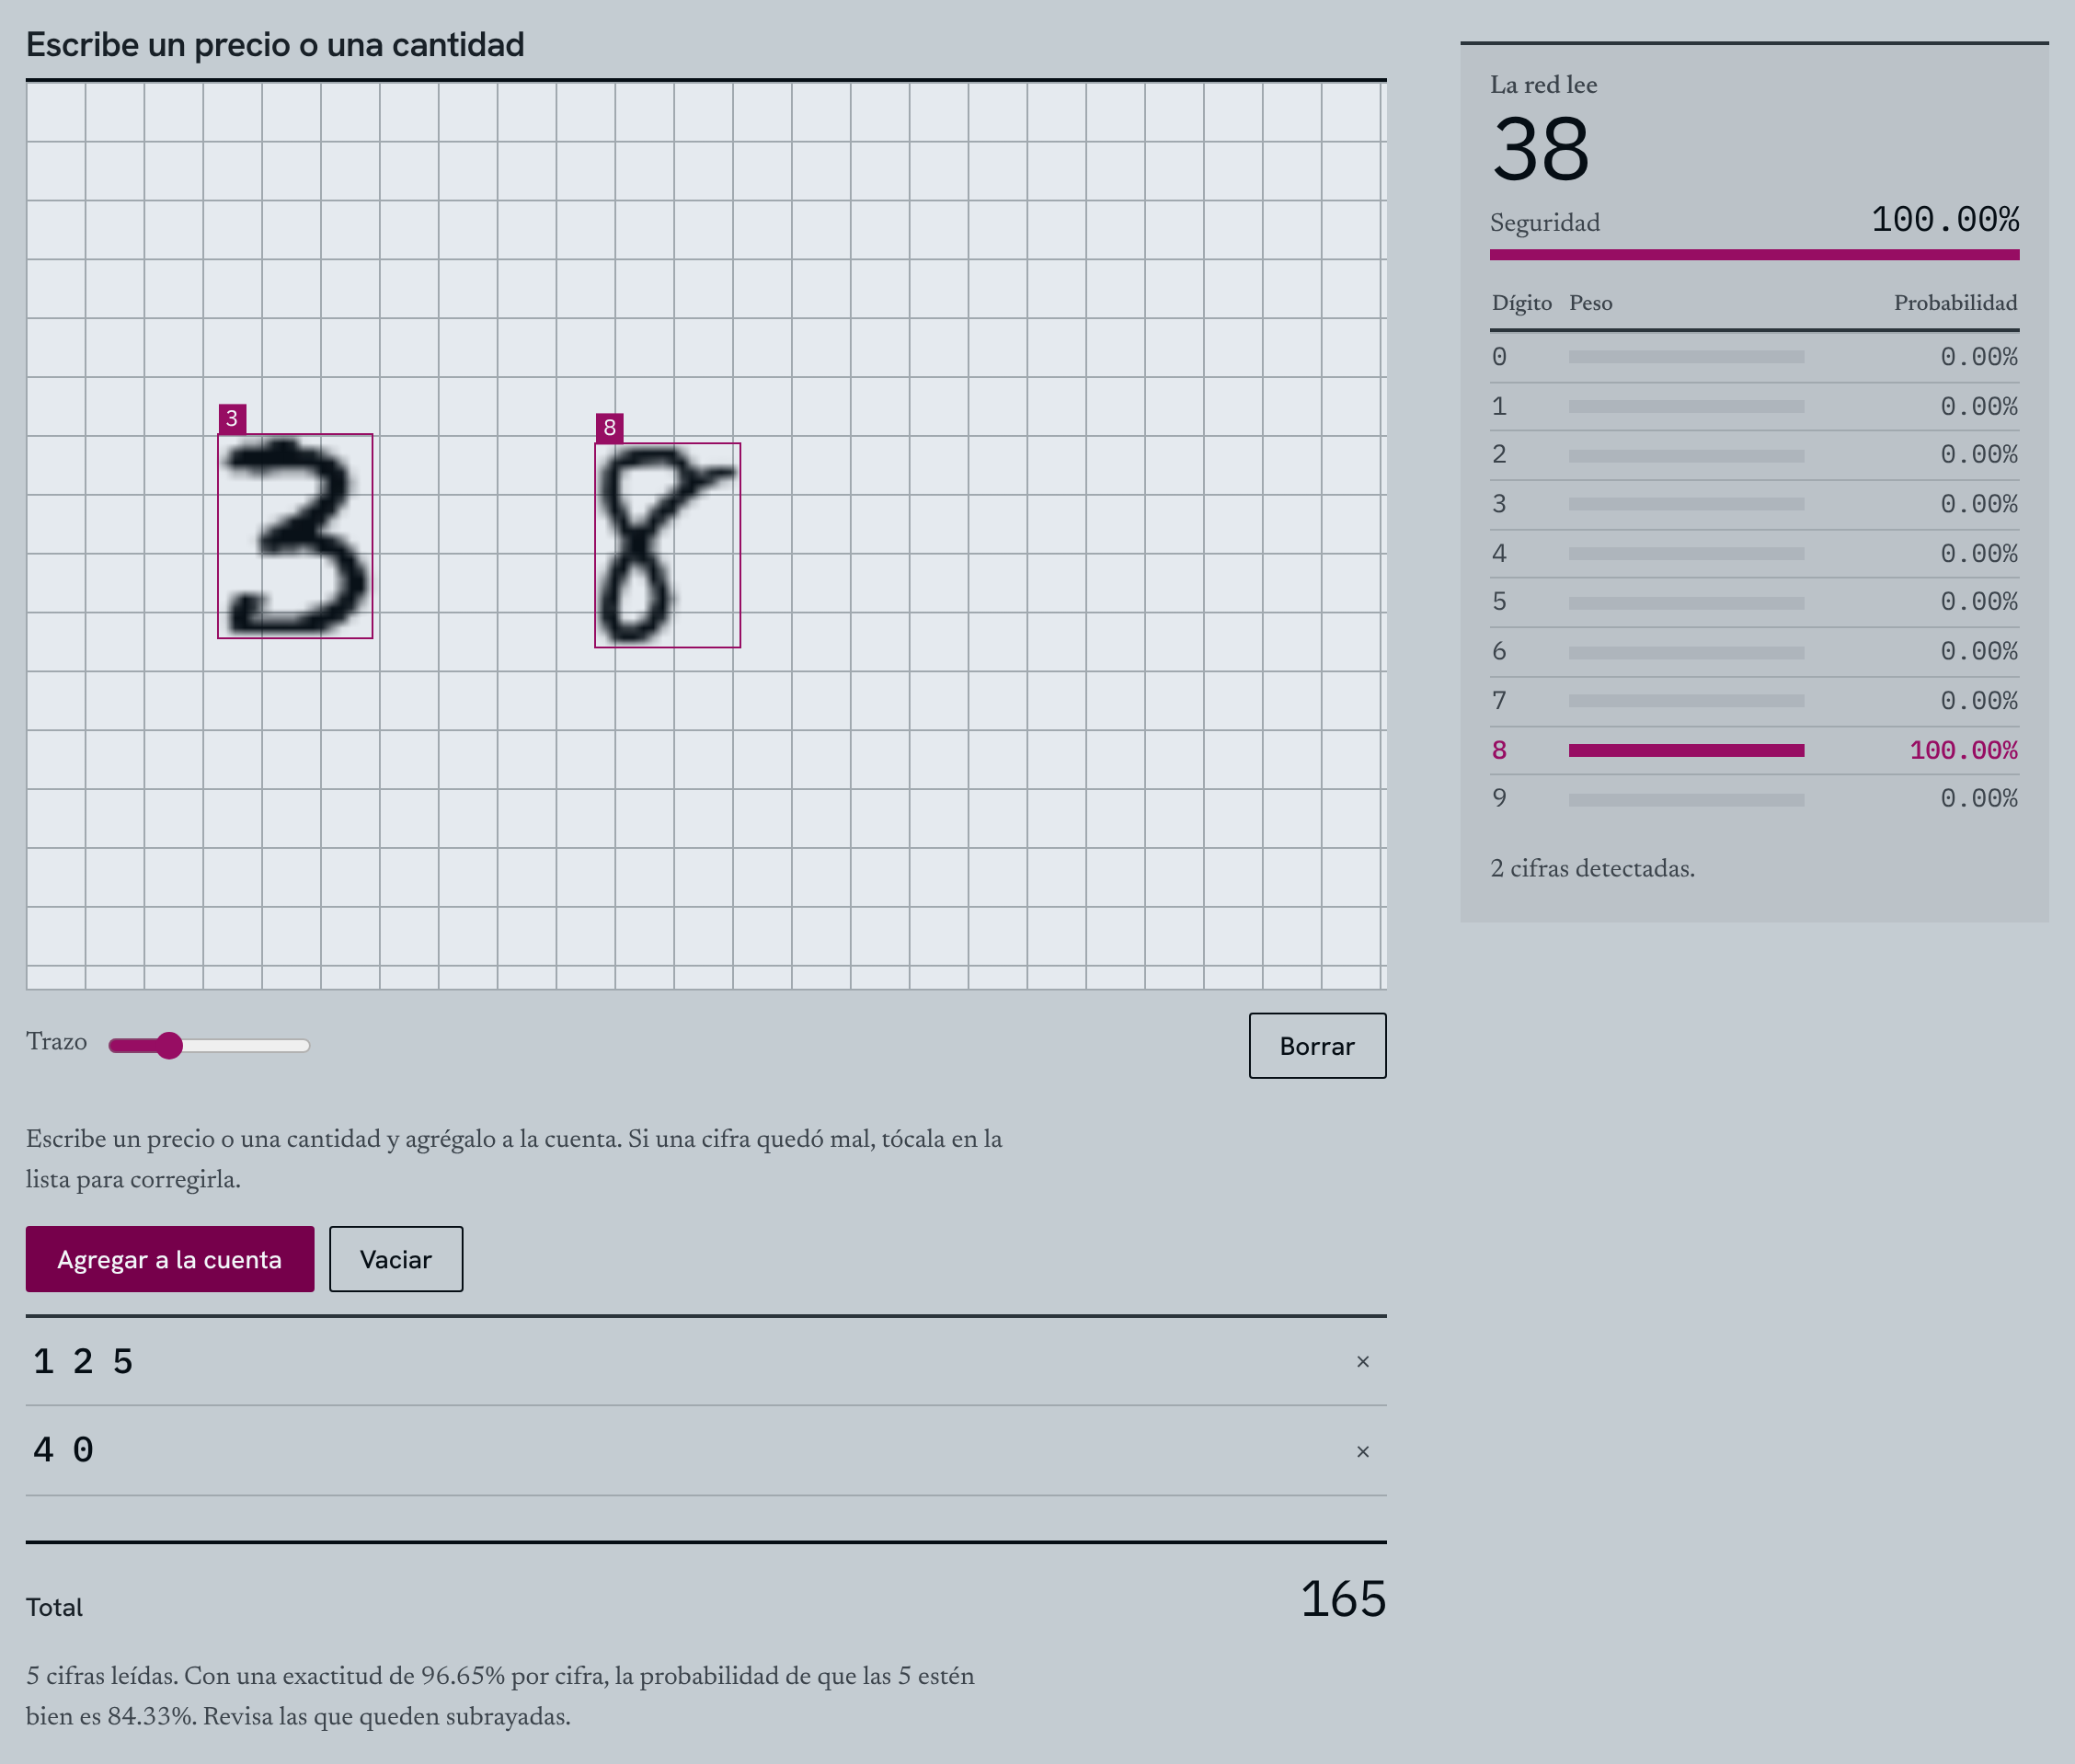
\includegraphics[width=\textwidth]{capturas/app-cuenta.png}
\caption{El modo de cuenta. A la izquierda, el lienzo con un número escrito y cada
cifra detectada encerrada en su propia caja; a la derecha, lo que la red lee y la
probabilidad que asigna a cada dígito. Abajo, los números ya agregados, el total y
el aviso de que, con cinco cifras leídas, la probabilidad de que todas estén bien es
$84.33\pc$.}
\label{fig:cuenta}
\end{figure}

\subsection{El panel de inspección}

El panel es el elemento que permite sustentar el funcionamiento interno y no solo el
resultado. Tiene cinco secciones:

\begin{description}[leftmargin=1.4em,style=nextline,itemsep=4pt]
\item[Capas] Muestra el diagrama de la red con cada neurona encendida según su
  activación con el dibujo actual, y al tocar una neurona dibuja sus conexiones más
  fuertes (Figura~\ref{fig:capas}).
\item[Neuronas] Muestra los pesos de cada neurona de la primera capa como una
  imagen de $28\times28$.
\item[Cálculo] Despliega la operación completa de la neurona seleccionada, término a
  término, con los números del dibujo que está en pantalla
  (Figura~\ref{fig:calculo}).
\item[Discreta] Contiene la matriz binaria, el conteo del espacio, la distancia de
  Hamming a cada dígito y la tabla de verdad
  (Figuras~\ref{fig:discretamatriz} y~\ref{fig:discretahamming}).
\item[Entrenar] Permite guardar dibujos propios y reentrenar la red en el navegador.
\end{description}

\begin{figure}[htbp]
\centering
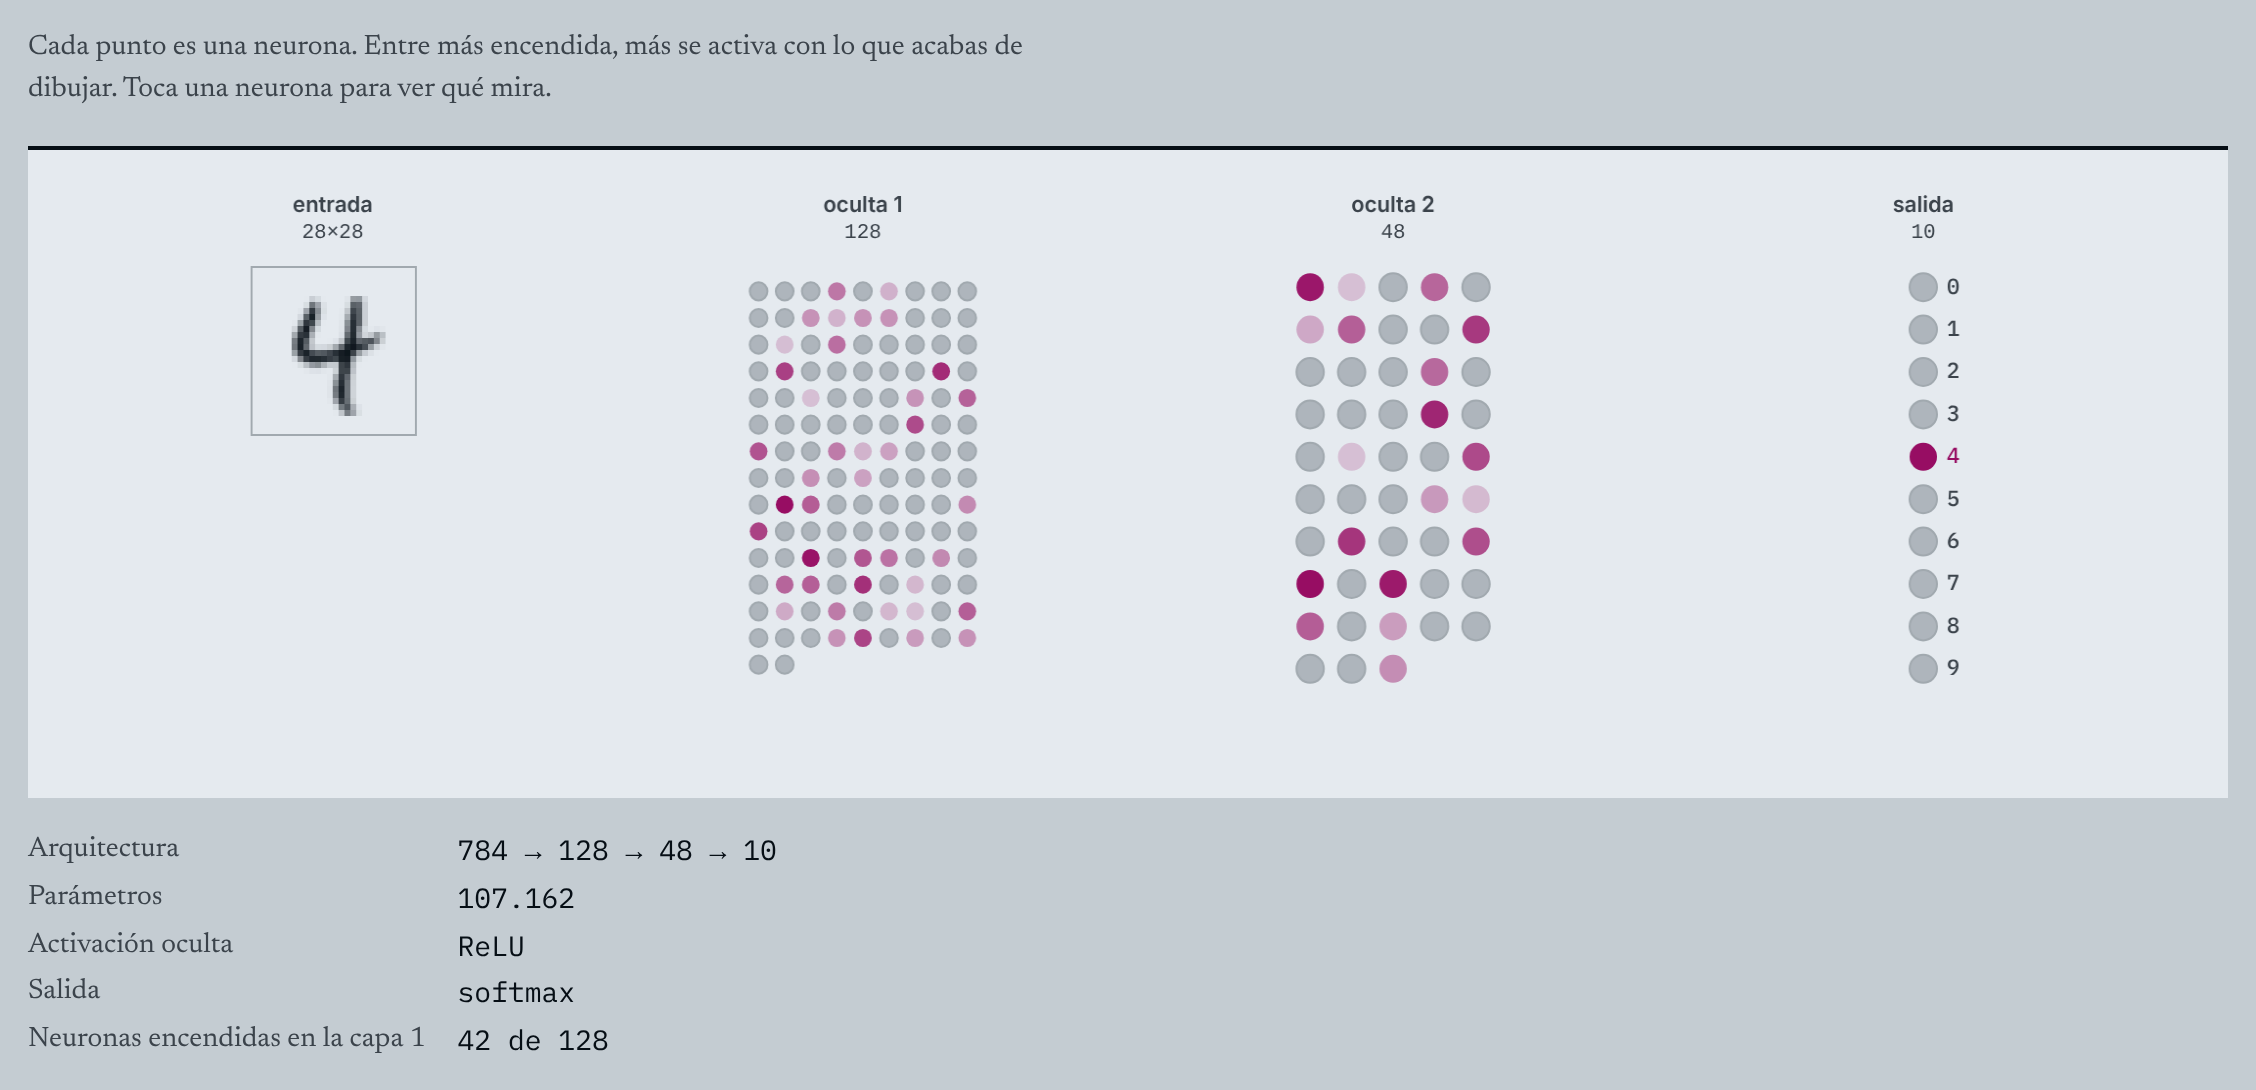
\includegraphics[width=\textwidth]{capturas/panel-capas.png}
\caption{La sección de capas con las neuronas activadas por el dibujo. De las 128
neuronas de la primera capa oculta, 42 se activan con este 4; las demás devuelven
cero.}
\label{fig:capas}
\end{figure}

\begin{figure}[htbp]
\centering
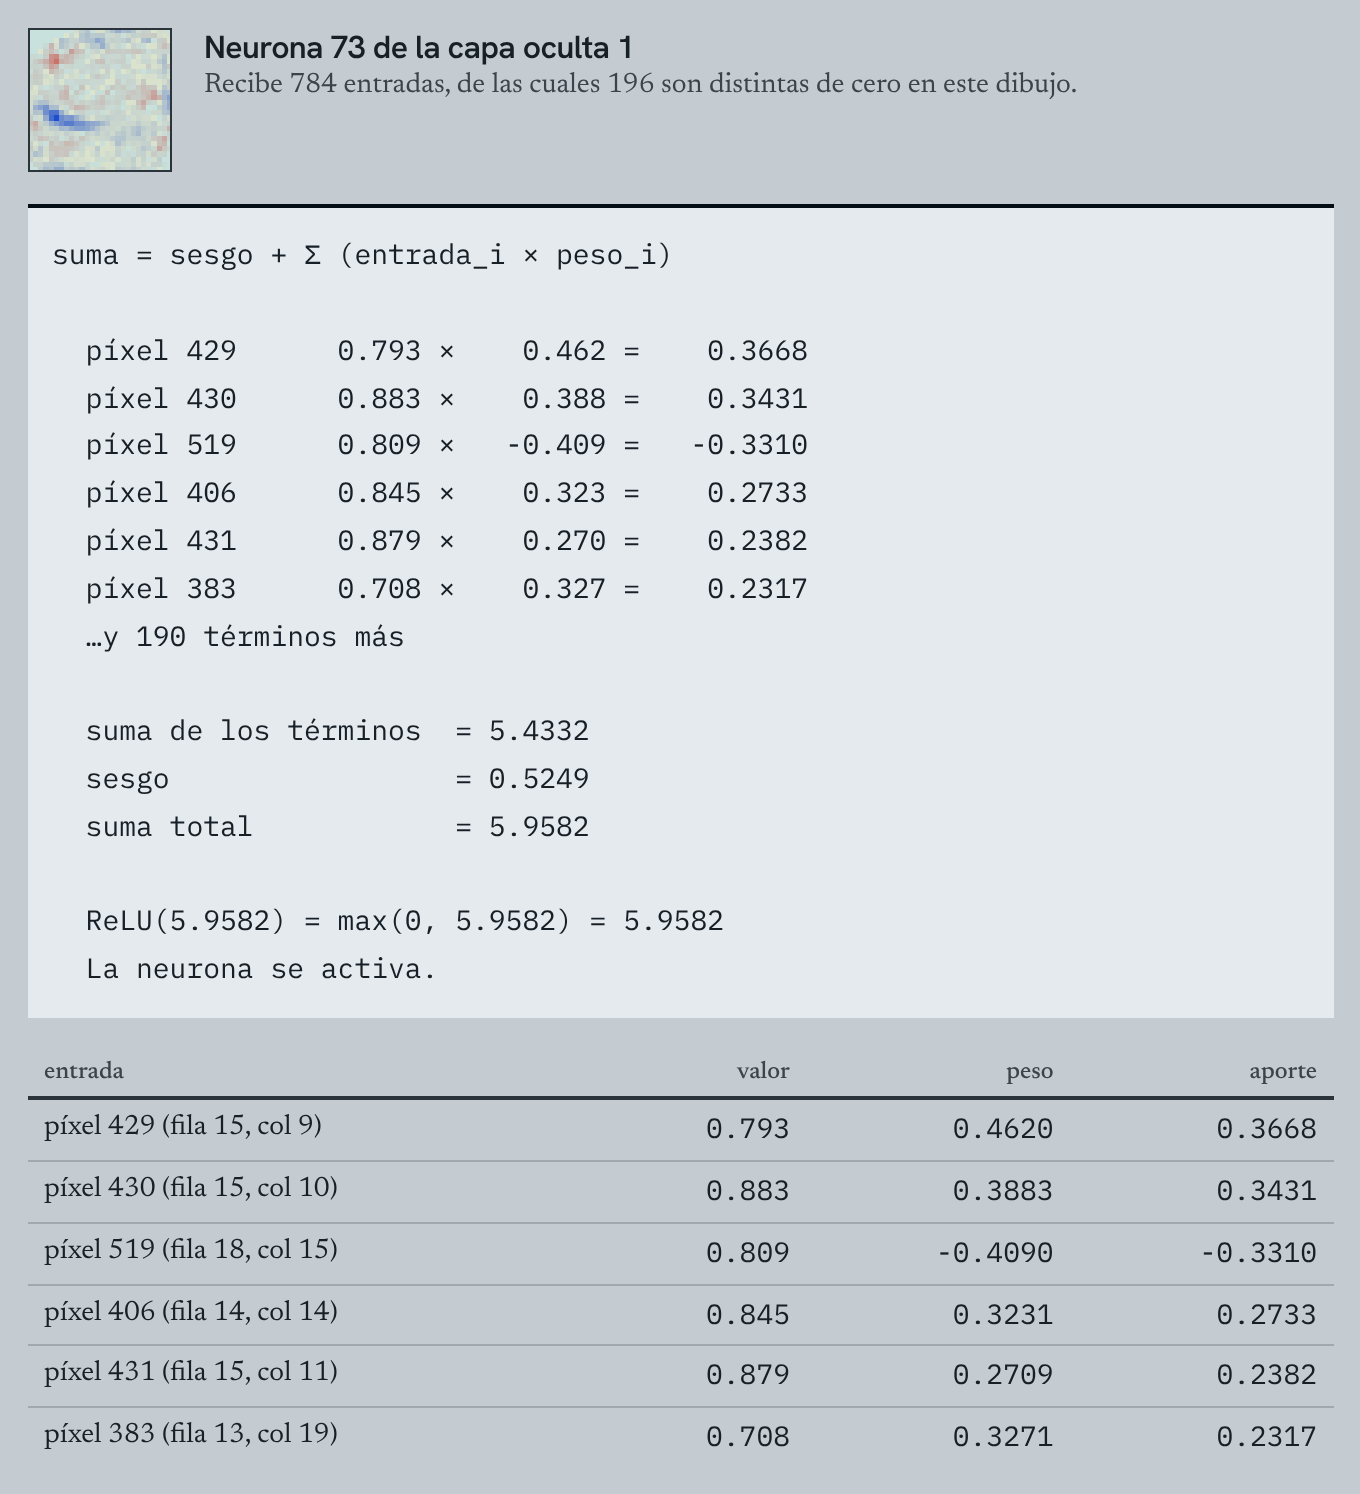
\includegraphics[width=0.86\textwidth]{capturas/panel-calculo.png}
\caption{La sección de cálculo: la suma ponderada de una neurona concreta, término a
término, con los valores del dibujo que está en pantalla, el sesgo, el total y el
resultado de aplicarle ReLU. No es un ejemplo ilustrativo; son los números que la
red está usando en ese momento.}
\label{fig:calculo}
\end{figure}

\begin{figure}[htbp]
\centering
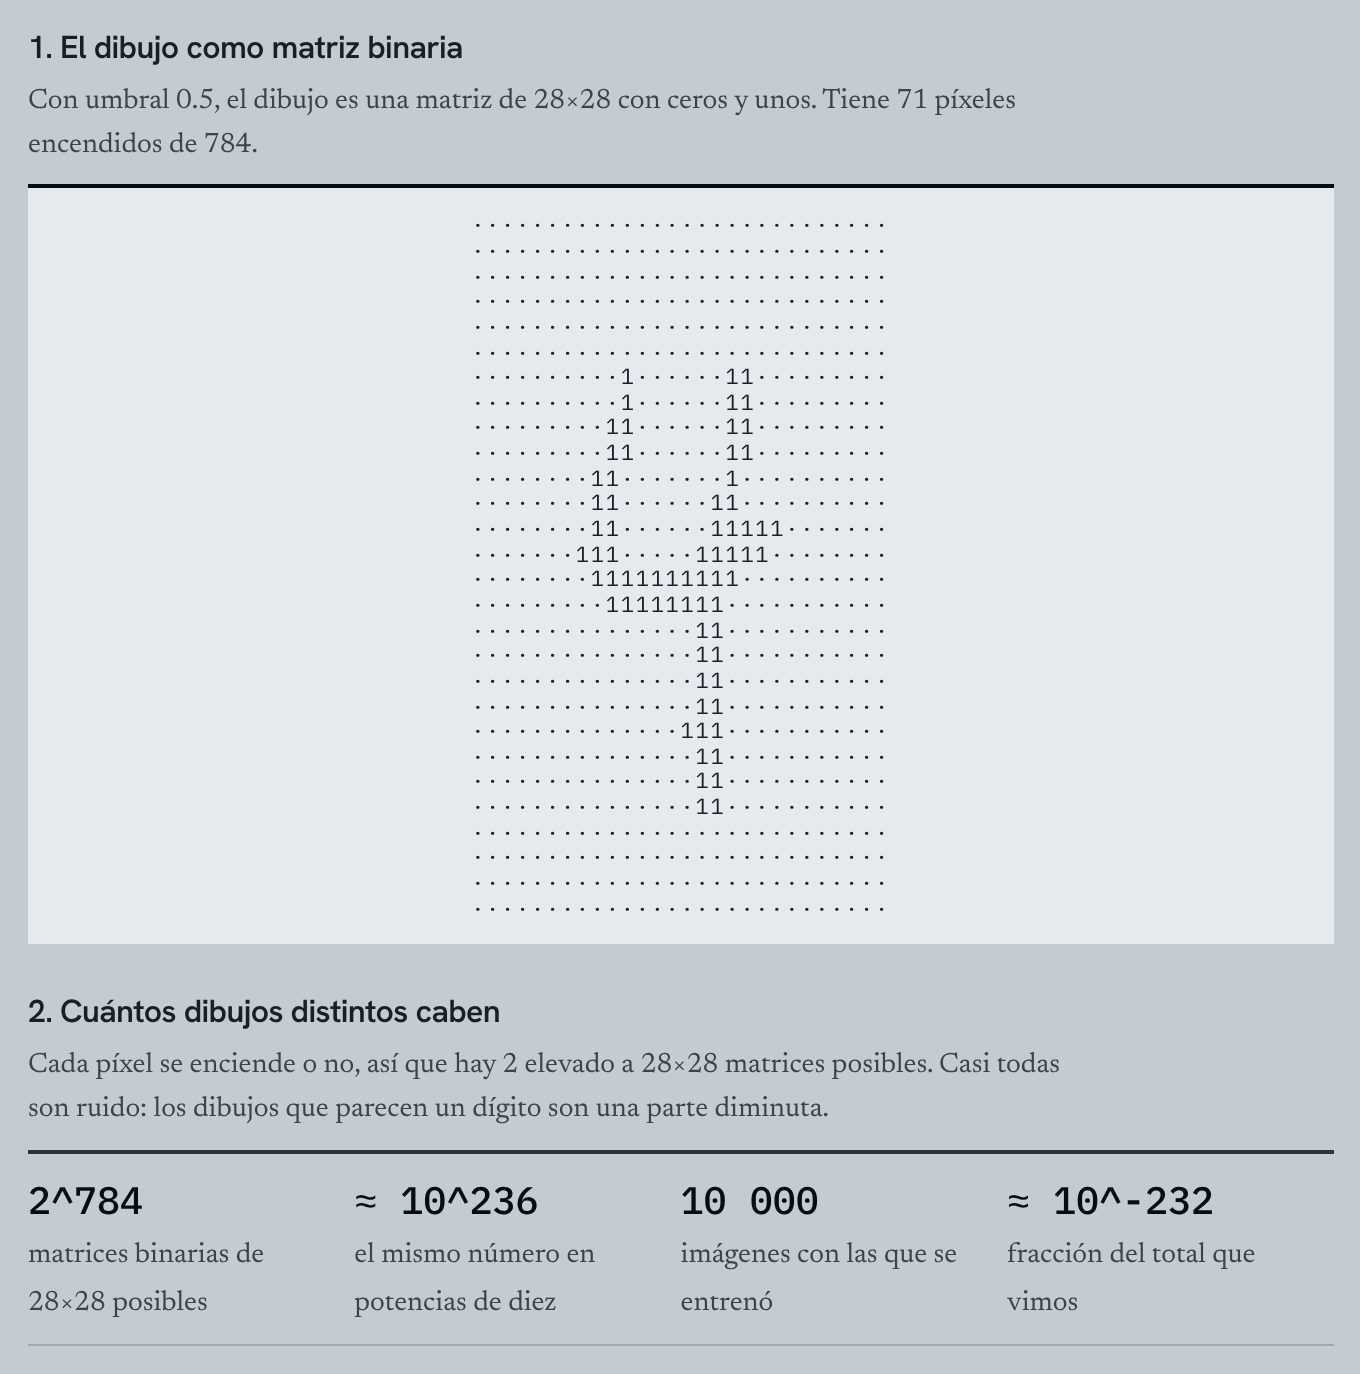
\includegraphics[width=0.86\textwidth]{capturas/panel-discreta-matriz.png}
\caption{La sección de matemática discreta, primera parte: el dibujo visto como
matriz binaria de $28\times28$ tras el umbral de $0.5$, y el conteo del espacio de
imágenes posibles con la fracción que el conjunto de datos representa.}
\label{fig:discretamatriz}
\end{figure}

\begin{figure}[htbp]
\centering
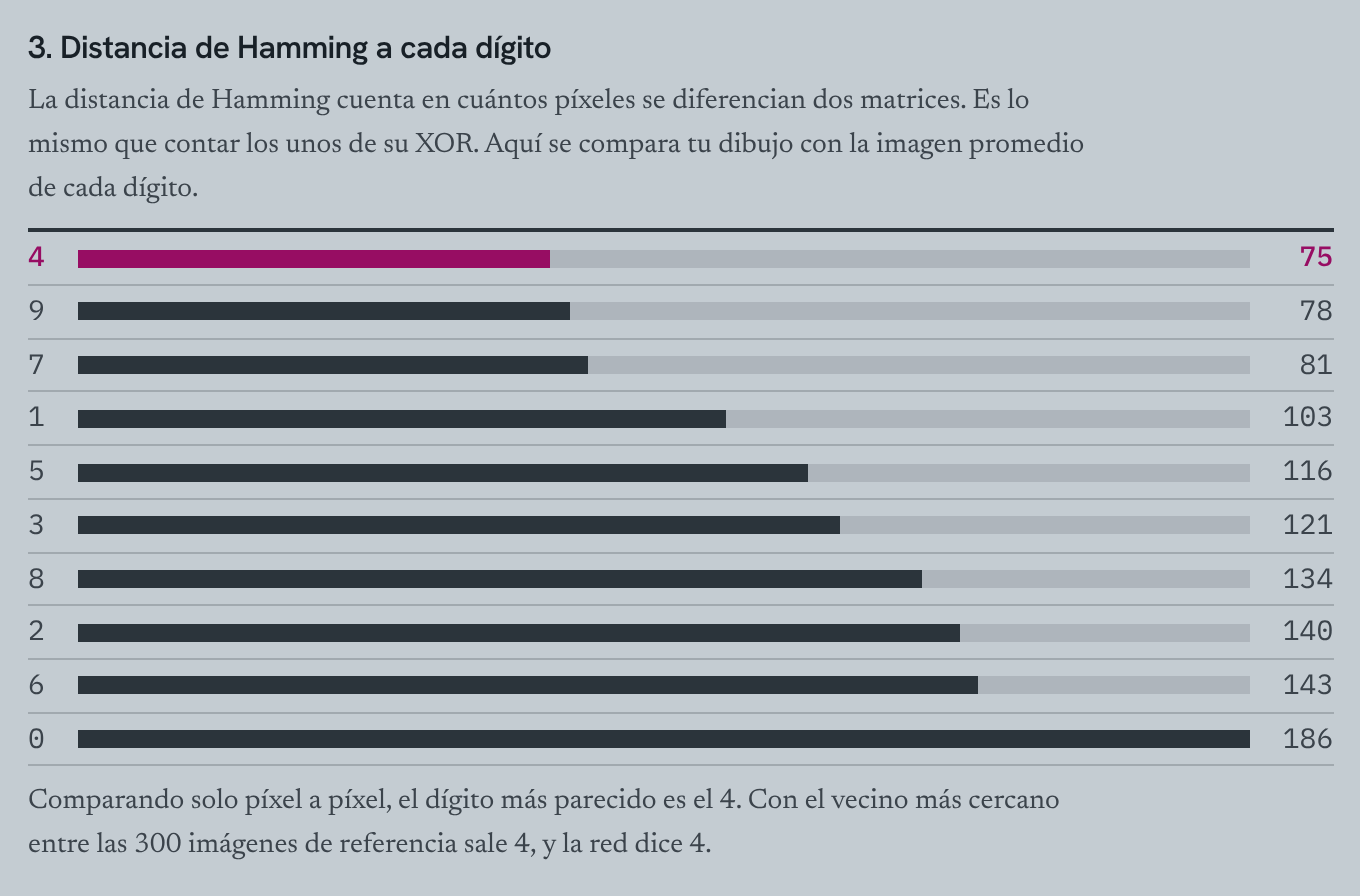
\includegraphics[width=0.86\textwidth]{capturas/panel-discreta-hamming.png}
\caption{La sección de matemática discreta, segunda parte: la distancia de Hamming
del dibujo a la imagen promedio de cada dígito, ordenada de menor a mayor, junto con
lo que responden el vecino más cercano y la red.}
\label{fig:discretahamming}
\end{figure}

Sobre el reentrenamiento conviene una precisión: si se entrenara únicamente con los
dibujos propios, la red olvidaría lo aprendido, fenómeno conocido como olvido
catastrófico. Para evitarlo, cada lote mezcla los dibujos nuevos con 300 imágenes de
referencia incluidas en la aplicación. Aun así, se trata de una demostración del
mecanismo y no de un entrenamiento serio, y los cambios no se conservan al recargar
la página.

Un hallazgo del panel merece mención, porque contradice la intuición. Es natural
esperar que los pesos de las neuronas se parezcan al dígito que detectan, pero no
ocurre, ni siquiera en un modelo de una sola capa. Los pesos no describen cómo es el
dígito, sino qué lo distingue de los otros nueve, y por eso se ven revueltos
(Figura~\ref{fig:plantillas}). Se intentó suavizar las plantillas aumentando la
regularización, y el resultado fue que la textura casi no cambia mientras la
exactitud cae de $90.45\pc$ a $81.35\pc$, de modo que se optó por explicar el
fenómeno en lugar de forzar la imagen.

\begin{figure}[htbp]
\centering
\includegraphics[width=\textwidth]{figuras/plantillas.pdf}
\caption{Arriba, la imagen promedio de cada dígito sobre el conjunto de
entrenamiento, que sí parece un dígito. Abajo, los pesos que aprende la regresión
logística sin capas ocultas para ese mismo dígito, que no. El rojo suma y el azul
resta: la neurona se activa cuando el trazo cae sobre el rojo y evita el azul.}
\label{fig:plantillas}
\end{figure}

La Figura~\ref{fig:neuronas} muestra el mismo fenómeno en la red final, y deja ver
además algo que conviene declarar: de las 128 neuronas de la primera capa oculta,
ocho no se activan con ninguna de las 2000 imágenes de prueba. Son neuronas muertas,
un efecto conocido de ReLU: una unidad cuya suma ponderada queda negativa para toda
entrada devuelve cero siempre y deja de recibir gradiente, de modo que conserva los
pesos aleatorios con que se inicializó. En la práctica significa que la red usa 120
de sus 128 neuronas y que la arquitectura tiene algo de holgura.

\begin{figure}[htbp]
\centering
\includegraphics[width=\textwidth]{figuras/neuronas.pdf}
\caption{Los pesos de las primeras 32 neuronas de la capa oculta, vistos como
imágenes de $28\times28$. Ninguna se parece a un dígito: cada una responde a un
trazo parcial. Las dos recuadradas en rojo, \texttt{n9} y \texttt{n27}, son neuronas
muertas; conservan el ruido de su inicialización porque nunca llegaron a activarse.}
\label{fig:neuronas}
\end{figure}

\subsection{Diseño de la interfaz}

La pantalla está organizada como una publicación de tablas y no como un tablero de
control: a la izquierda la hoja donde se escribe, a la derecha un registro que
muestra el número leído y los diez dígitos con su probabilidad, alineados al
decimal, con la fila ganadora destacada. La elección responde a lo que la aplicación
es: un instrumento que produce cifras. Funciona en computador, celular y tableta,
con tema claro y oscuro.

% ------------------------------------------------------------------ discusión --
\section{Discusión}

El resultado central del proyecto no es la exactitud de $96.65\pc$, sino la distancia
entre los cuatro modelos de la Tabla~\ref{tab:modelos}, porque esa distancia es la
que se explica con matemática discreta. Entre el clasificador trivial y el vecino más
cercano en Hamming hay $75.55$ puntos, y toda esa ganancia proviene de una idea
discreta: contar en cuántas posiciones difieren dos matrices binarias. Entre Hamming
y la regresión logística hay $3.65$ puntos, que provienen de aprender qué píxeles
importan y cuáles no. Y entre la regresión logística y la red hay $6.20$ puntos, que
provienen de poder combinar trazos parciales, es decir, exactamente de lo que una
sola capa no puede hacer, como demuestra el caso de XOR.

Dicho de otro modo, el apartado~\ref{sec:xor} no es un adorno teórico: el salto de
$90.45\pc$ a $96.65\pc$ es el precio que se paga por no tener capas ocultas, medido
sobre este problema concreto.

Un segundo punto de discusión es el papel del aumento de datos frente al tamaño del
modelo. En la primera comparación, duplicar las neuronas de 32 a 64 mejoró la
validación en $0.07$ puntos, una diferencia despreciable. La mejora real, de $1.70$
puntos, llegó al generar variantes de las imágenes que imitan cómo varía la escritura
humana. Esto sugiere que la limitación del proyecto no estaba en la capacidad del
modelo sino en la cantidad y variedad de los datos, lo que es coherente con haber
usado 10\,000 de las 70\,000 imágenes disponibles en MNIST.

Un tercer punto es la diferencia entre acertar y ser útil. Las
Tablas~\ref{tab:calibracion} y~\ref{tab:kcifras} muestran que una exactitud por cifra
que parece alta se traduce en un error cada ocho números de cuatro cifras.
Reconocerlo cambió el diseño de la aplicación: en lugar de presentar un total y
confiar en él, el modo de cuenta expone cada cifra y facilita corregirla. Un sistema
honesto sobre su incertidumbre resulta más utilizable que uno que la esconde.

% --------------------------------------------------------------- limitaciones --
\section{Limitaciones}

Se declaran de forma explícita las siguientes limitaciones.

\begin{itemize}
\item El conjunto de datos contiene dígitos escritos con lápiz por adultos y
  estudiantes estadounidenses. Un trazo de dedo sobre una pantalla es distinto, de
  modo que la exactitud real de uso puede ser menor que el $96.65\pc$ medido.
\item Se emplearon 10\,000 de las 70\,000 imágenes de MNIST, por la vía de obtención
  descrita en el apartado~\ref{sec:datos}.
\item La aplicación no se ha probado de forma sistemática con usuarios reales
  escribiendo con el dedo, ni con niños ni con comerciantes. Las pruebas
  automatizadas dibujan imágenes del conjunto de datos sobre el lienzo.
\item El panel muestra lo que la red hace, no lo que entiende. Cuando se afirma que
  una neurona responde a cierto trazo, se trata de una lectura de sus pesos y no de
  una afirmación sobre lo que la neurona representa.
\item Ocho de las 128 neuronas de la primera capa oculta no se activan con ninguna
  imagen de prueba. No afectan el resultado medido, pero indican que la arquitectura
  podría ser algo menor sin perder exactitud.
\item El reentrenamiento dentro del navegador usa pocos ejemplos y sirve para
  demostrar el mecanismo; no constituye un entrenamiento válido y sus cambios no
  persisten.
\item El reconocimiento de operaciones completas con signos de suma, resta,
  multiplicación e igualdad quedó fuera del alcance de esta entrega, por requerir la
  recolección de muestras propias de cada signo.
\item El análisis de importancia de los píxeles de entrada es aproximado, por la
  razón combinatoria expuesta en el apartado~\ref{sec:combinatoria}, y no captura las
  interacciones entre ellos.
\end{itemize}

% --------------------------------------------------------------- conclusiones --
\section{Conclusiones}

Se construyó una aplicación web que reconoce dígitos escritos a mano con una exactitud
de $96.65\pc$ sobre un conjunto de prueba independiente, superando en $6.20$ puntos a
un modelo lineal y en $9.85$ puntos a un clasificador puramente discreto basado en la
distancia de Hamming.

El problema admite una formulación completa en términos de matemática discreta. La
imagen es una matriz binaria de $28\times28$; las operaciones entre dibujos son
operaciones booleanas; la diferencia entre dos dibujos es la distancia de Hamming,
que coincide con el peso de su disyunción exclusiva; el espacio de dibujos posibles
tiene cardinalidad $2^{784}$ y el conjunto observado es una fracción del orden de
$10^{-232}$ de ese total; y la relación de representar el mismo dígito es de
equivalencia y lo parte en diez clases.

La necesidad de capas ocultas quedó justificada de dos maneras independientes y
concordantes: de forma teórica, porque de las 16 funciones booleanas de dos variables,
14 son linealmente separables y la disyunción exclusiva no lo es, lo que obliga a
componer funciones; y de forma empírica, porque el modelo sin capas ocultas se queda
$6.20$ puntos por debajo de la red sobre este mismo problema.

El aumento de datos resultó más determinante que el tamaño del modelo. Las
transformaciones que imitan la variación natural de la escritura aportaron una mejora
de $1.70$ puntos, mientras que duplicar el número de neuronas sin cambiar los datos
aportó $0.07$.

El preprocesado del trazo resultó ser una pieza crítica y no un detalle de
implementación. Replicar sobre el dibujo del usuario la misma normalización que traen
los datos de entrenamiento cuesta $0.33$ puntos de exactitud y, a cambio, hace que la
lectura sea prácticamente independiente de dónde y de qué tamaño se escriba.

Finalmente, la reimplementación de la red en el navegador, verificada contra la
versión de Python, permite exhibir el funcionamiento interno del modelo en tiempo
real. Esto convierte el proyecto en un instrumento de explicación y no solo en un
clasificador, que era el objetivo buscado para la asignatura.

% ---------------------------------------------------------------- referencias --
\section{Referencias}

\begin{description}[leftmargin=1.5em,style=unboxed,itemsep=5pt,labelsep=0pt,font=\normalfont]
\item Cazala, J. (2016). \textit{mnist} [Paquete de software]. npm, licencia MIT.
  \url{https://github.com/cazala/mnist}
\item LeCun, Y., Cortes, C. y Burges, C. J. C. (1998). \textit{The MNIST database of
  handwritten digits}. \url{http://yann.lecun.com/exdb/mnist/}
\item Pedregosa, F., Varoquaux, G., Gramfort, A., Michel, V., Thirion, B., Grisel, O.,
  \dots\ Duchesnay, É. (2011). Scikit-learn: Machine learning in Python.
  \textit{Journal of Machine Learning Research, 12}, 2825--2830.
\item Rosen, K. H. (2019). \textit{Discrete mathematics and its applications}
  (8.\textsuperscript{a} ed.). McGraw-Hill Education.
\end{description}

\vspace{0.6em}
\noindent Repositorio del proyecto: \url{https://github.com/SZelaya08/Cifra}

\noindent Aplicación en funcionamiento: \url{https://szelaya08.github.io/Cifra/}

% -------------------------------------------------------------------- anexos --
\appendix

\section{Reproducibilidad}

Todo el experimento es reproducible con semilla fija 42. Los comandos, en orden, son
los siguientes.

\begin{quote}\ttfamily\small
python3 -I preparar\_datos.py ../datos/mnist10k.npz ../resultados\\
python3 -I entrenar.py ../datos/split\_28x28.npz ../resultados\\
python3 -I mejorar.py ../datos/split\_28x28.npz ../resultados\\
python3 -I exportar.py ../datos/split\_28x28.npz ../resultados ../docs\\
python3 -I discreta.py ../datos/split\_28x28.npz ../resultados
\end{quote}

Las verificaciones se ejecutan sobre Node: \texttt{validar\_red.mjs} comprueba que la
red de JavaScript coincide con la de Python, \texttt{validar\_preproceso.mjs} mide el
efecto del preprocesado y \texttt{probar\_app.mjs} abre la aplicación en un navegador
real y corre 26 comprobaciones de funcionamiento, que pasan en escritorio y en
celular, con tema claro y oscuro.

\section{Estructura del repositorio}

\begin{description}[leftmargin=2.6em,style=nextline,itemsep=3pt,font=\ttfamily]
\item[docs] La aplicación web, que es lo que publica GitHub Pages.
\item[codigo] Los programas de Python que preparan los datos, entrenan, evalúan,
  exportan y calculan la parte discreta, y los programas de Node que verifican.
\item[datos] El conjunto de imágenes y la partición de entrenamiento y prueba.
\item[resultados] Las métricas en formato JSON y las figuras generadas.
\item[capturas] Las capturas de pantalla de la aplicación.
\item[BITACORA.md] El registro de cada tarea con sus decisiones, que es la fuente de
  este informe.
\end{description}

\clearpage
\section{Precisión y exhaustividad por dígito}
\label{ap:pordigito}

La Tabla~\ref{tab:pordigito} presenta la precisión, la exhaustividad y el valor F1 de
la red final para cada dígito, sobre el conjunto de prueba de 2000 imágenes. Los
valores provienen de \texttt{resultados/t09b\_mejora.json}.

% Sin entorno flotante: esta tabla tiene que quedar donde está escrita, justo
% debajo del párrafo que la presenta, y no al principio de la página siguiente.
\begin{center}
\captionof{table}{Precisión, exhaustividad y F1 por dígito sobre el conjunto de
prueba. La última columna es el número de imágenes de esa clase presentes en el
conjunto de prueba; las diez suman 2000.}
\label{tab:pordigito}
\begin{tabular}{crrrr}
\toprule
\textbf{Dígito} & \textbf{Precisión} & \textbf{Exhaustividad} & \textbf{F1} & \textbf{Imágenes} \\
\midrule
0 & 0.9849 & 0.9800 & 0.9824 & 200 \\
1 & 0.9739 & 0.9955 & 0.9846 & 225 \\
2 & 0.9790 & 0.9444 & 0.9614 & 198 \\
3 & 0.9439 & 0.9805 & 0.9619 & 206 \\
4 & 0.9841 & 0.9489 & 0.9662 & 196 \\
5 & 0.9534 & 0.9479 & 0.9507 & 173 \\
6 & 0.9521 & 0.9802 & 0.9660 & 203 \\
7 & 0.9543 & 0.9766 & 0.9653 & 214 \\
8 & 1.0000 & 0.9365 & 0.9672 & 189 \\
9 & 0.9450 & 0.9642 & 0.9545 & 196 \\
\midrule
\multicolumn{4}{r}{\textit{Total}} & \textbf{2000} \\
\bottomrule
\end{tabular}
\end{center}

\noindent La precisión responde a «de todo lo que la red leyó como este dígito, cuánto lo era
de verdad», y la exhaustividad a «de todos los ejemplos de este dígito, cuántos
encontró». La precisión de $1.0000$ del dígito 8 no es un error de cálculo: significa
que ninguna otra cifra fue leída nunca como un 8. El 8 pierde por exhaustividad
---\,su $0.9365$ es el más bajo de la tabla\,--- porque a veces se lee como 6 o como 5,
que es lo que recoge la Tabla~\ref{tab:pares}.

\end{document}
